\chapter{A Point-Classification Neural Network}
%\usepackage{amsfonts}
%\usepackage{amsmath}
%\usepackage{graphicx}
%\usepackage{listings}

\section{Introduction}
In this article we implement a simplest neural network with python 3. This implementation is mainly for learning and understanding, without a regularization term and any use of existing deep learning framework.

\subsection{What's A Point-classification Neural Network}
Suppose we draw a curve on a canvas, which separates the canvas, or every point on it, into several classes. Now, suppose we have only finite points and their classes, we want to reconstruct the curve. The reconstruction is done by a neural network, trained with the given points. We use it to predict the class of every point on the canvas, and the boundary of the different classes points is the curve we want.
\begin{center}
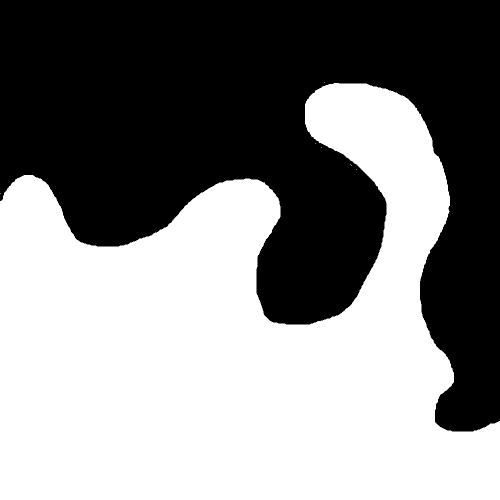
\includegraphics[width=0.3\textwidth]{figures/pcNN_train3.png}
\end{center}

\subsection{What Does the Neural Network Look Like}
Viewed as a function $f$, the neural network can be written as
\[f(x)=L_3\circ L_2\circ L_1(x)\]
where $x$ denotes the input vector,  $L_1$ and $L_2$ denote the two hidden layers, and $L_3$ denotes the output layer.
\begin{center}
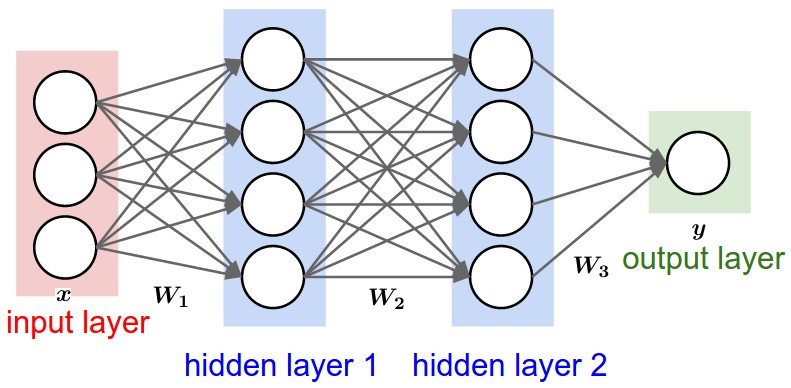
\includegraphics[width=0.5\textwidth]{figures/pcNN_Fig2}
\end{center}

\subsection{Mathematical Expression of Each Part}
The neural network is \[f(x)=y,\quad x,y\in\mathbb{R}^2,\]
and the loss function is \[L(y)=\frac{1}{2}\|y-p\|^2=\frac{1}{2}\sum_{i=1}^2{(y_i-p_i)^2}\]
where $p$ is the true classification vector.\\
$f(x)=L_3\circ L_2\circ L_1(x)$, where
\[
\begin{split}
L_1(x)=A(xW_1+b_1)=\frac{1}{1+e^{-(xW_1+b_1)}}\in\mathbb{R}^{10},\\
x\in\mathbb{R}^{2},W_1\in\mathbb{R}^{10\times2},b_1\in\mathbb{R}^{10},
\end{split}
\]
\[
\begin{split}
L_2(x)=A(xW_2+b_2)=\frac{1}{1+e^{-(xW_2+b_2)}}\in\mathbb{R}^{10},\\
x\in\mathbb{R}^{10},W_2\in\mathbb{R}^{10\times10},b_2\in\mathbb{R}^{10},
\end{split}
\]
\[
\begin{split}
L_3(x)=A(xW_3+b_3)=\frac{1}{1+e^{-(xW_3+b_3)}}\in\mathbb{R}^{2},\\
x\in\mathbb{R}^{10},W_3\in\mathbb{R}^{2\times10},b_3\in\mathbb{R}^{2}.
\end{split}
\]
Each column of the matrix $W_i$ represents a neuron in the layer $i$. So, layer $1$ has $10$ neurons, layer $2$ has $10$ neurons, and layer $3$ has $2$ neurons.\\

\subsection{What Does A Digital Picture Look Like}
The input picture will first be transformed into a grey-scale picture. Then, the values of pixels correspond to a matrix, and we have a matrix as our picture.

\begin{center}
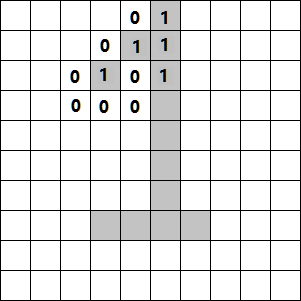
\includegraphics[width=0.5\textwidth]{figures/pcNN_mesh.png}
\end{center}

\section{The Implementation}
\subsection{Produce Training Data}

\subsection{Produce A Training Curve}

To give such a curve, or picture, for example, one can draw it by \emph{paint} on windows, or any other tools on different platforms.\\
If you use \emph{paint}, save it as \emph{train.png} and use the following to load it.

\begin{lstlisting}
from PIL import Image
import numpy as np
pil_im = Image.open('train.png').convert('L')
data = np.asarray(pil_im)
\end{lstlisting}

This will load the picture in \emph{pil\_im}, and transform it into an array \emph{data}. Now, each element of \emph{data} corresponds to the grey scale of a pixel.\\

\section{Generate A Training Dataset}

To get a training dataset, we generate a couple of coordinates randomly. We then generate the classification from the picture, and scale the dataset by dividing its length.

\subsection{Backward Propagation}
\subsubsection{Backward Propagation (BP) in A Layer}
Viewed as a unity, a layer will carry out the follows.
\begin{itemize}
\item Recive an input row vector $x$
\item Compute $y=xW+b$
\item Send $A(y)=\frac{1}{1+e^{-y}}$ to the next layer
\end{itemize}
In BP, We want to update $W$ and $b$ by the gradient descent method.\\
We already have a loss function $L$, and we know the update process is
\[W = W + \delta D_WL,\]
\[b = b+\delta D_bL.\]
Let's figure out how to compute $D_WL$ and $D_bL$.

\subsubsection{Backward Propagation (BP) in A Layer, Update W}
Let $W_i$ be the $i$th column of W, we have
\[\nabla_{W_i}L=D_{W_i}L=\partial_{y_i}L\nabla_{W_i}y_i\]
as a cloumn vector. We then have
\[
\begin{split}
D_WL&=
\begin{pmatrix} \nabla_{W_1}L & \dots & \nabla_{W_m}L
\end{pmatrix}\\
&=
\begin{pmatrix}
\partial_{y_1}L & \dots &\partial_{y_m}L
\end{pmatrix}
\times
\begin{pmatrix}
\nabla_{W_1}y_1 & \dots & \nabla_{W_m}y_m
\end{pmatrix}
\end{split}
\]
where the multiplication is element-wise.
We know that
\[
\nabla_{W_i}y_i=\nabla_{W_i}{(xW_i+b_i)}=x^T.
\]
Thus we have
\[
D_WL=x^T
\begin{pmatrix}
\partial_{y_1}L & \dots &\partial_{y_m}L
\end{pmatrix}.
\]

\subsubsection{Backward Propagation (BP) in A Layer, Update b}
Very similar to $W$, we update $b_i$ by
\[\partial_{b_i}L=\partial_{y_i}L\nabla_{b_i}y_i=\partial_{y_i}L.\]
So we have
\[D_bL=
\begin{pmatrix}
\partial_{y_1}L & \dots &\partial_{y_m}L
\end{pmatrix}.
\]
Now we show how to compute
\[
D_yL=\nabla_yL=
\begin{pmatrix}
\partial_{y_1}L & \dots &\partial_{y_m}L
\end{pmatrix}.
\]
Basically, one should follow the steps below.
\begin{itemize}
\item When you are in a hidden layer, just call the next layer to make it send $\nabla_yL$ to you.
\item If the prior layer asked you for $\nabla_{\hat y}L$, follow the steps below.
\end{itemize}
By the chain rule we have
\[
\nabla_{\hat y}L=D_{y}L\cdot D_xy\cdot D_{\hat y}x.
\]
We have already get $D_yL$. For the rest two, we have
\[
D_xy_i=\nabla_xy_i=\nabla_x(xW_i+b_i)=W_i^T,
\]
so we have
\[
D_xy=
\begin{pmatrix}
W_1^T \\ \dots\\ W_m^T
\end{pmatrix}
=W^T
\]

On the other hand,
\[
D_{\hat y}x_i=D_{\hat y}A({\hat y}_i)=(1-{\hat y}_i){\hat y}_i1_i,
\]
so we have
\[
D_{\hat y}x=D_{\hat y}A({\hat y}_i)=\text{diag}{((1-{\hat y}_i){\hat y}_i)}.
\]
As a result, we have
\[
\begin{split}
D_{\hat y}L&=D_yL\cdot
\begin{pmatrix}
W_1^T(1-{\hat y}_1){\hat y}_1 \\ \dots\\ W_m^T(1-{\hat y}_m){\hat y}_m
\end{pmatrix}\\
&=(D_yL\times
\begin{pmatrix}
(1-{\hat y}_1){\hat y}_1 & \dots & (1-{\hat y}_m){\hat y}_m
\end{pmatrix})
\cdot W^T\\
&=(D_yL\times(1-{\hat y}){\hat y})\cdot W^T
\end{split}.
\]



When you are in the last layer, there's no next layer to call. What we need is
\[
\nabla_yL=
\begin{pmatrix}
\partial_{y_1}L & \dots &\partial_{y_m}L
\end{pmatrix}.
\]
Our loss function is
\[
L(y)=\frac{1}{2}\sum_i{(y_i-p_i)}^2,
\]
so we have
\[
\nabla_yL=
\begin{pmatrix}
y_1-p_1 & \dots & y_n-p_n
\end{pmatrix}
\]
where $n$ is the number of classes.

We propagate only one vector $x$ in the above discussions, which is not efficient. Now we want to propagate a \emph{batch} of $x$, denote as a matrix $X$, with each row an input vector.
\begin{itemize}
    \item When update $W$ and $b$, we just sum up the gradients to get our new gradients,
\[W = W + \delta\sum_i D_WL(X_i)=W+\delta\Delta W,\]
\[b = b+\delta\sum_i D_bL(X_i)=b+\delta\Delta b.\]
where $X_i$ denotes the $i$th row of $X$, and $\delta$ is the step size.
\end{itemize}

This can be rewritten as
\[
\Delta W=X^T\nabla_yL,
\]
\[
\Delta b=1^T\nabla_yL.
\]
We now finished the backforward propagation
\[
W=W+\delta X^T\nabla_yL
\]
\[
b=b+\delta 1^T\nabla_yL
\]
\[
D_{\hat y}=(D_yL\times(1-{\hat y}){\hat y})\cdot W^T
\]
A note for batches. We can choose a batch, i.e. a subset of dataset randomly, and update them at one time. After this, we do this again, until the result is acceptable.


\subsection{The Step Size $\delta$}

Fixed step size and others like optimal step size show different performance in decreasing the loss function.
\begin{center}
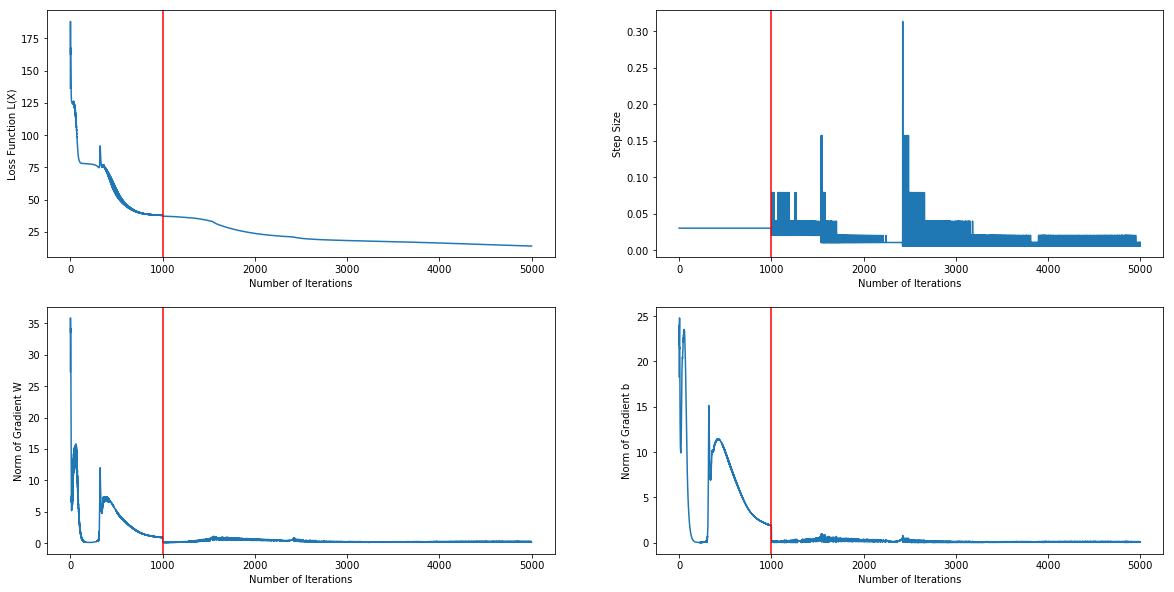
\includegraphics[width=\textwidth]{figures/pcNN_a2.png}
\end{center}
